\documentclass{article}
\usepackage{tikz}
\usetikzlibrary{arrows.meta,positioning,calc,shapes.geometric}
\pagestyle{empty}
\begin{document}
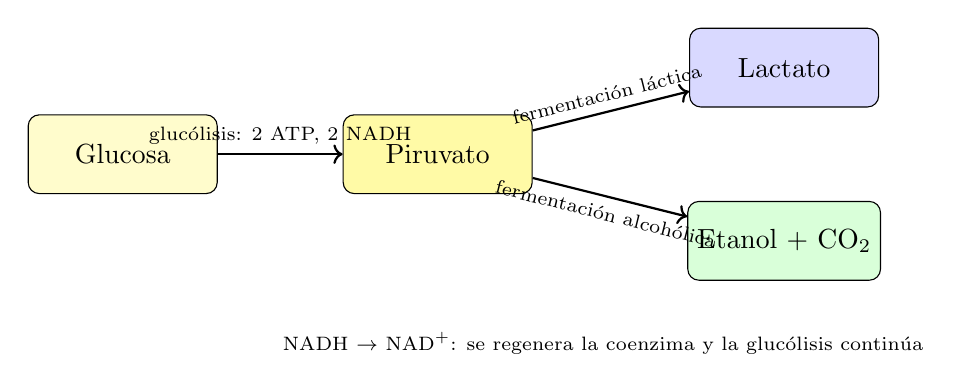
\begin{tikzpicture}

\def\bx#1#2#3#4{\node[draw, rounded corners, fill=#4, minimum width=2.4cm, minimum height=1.0cm, align=center] (#1) at (#2) {#3};}
\bx{g}{0,0}{Glucosa}{yellow!20}
\bx{p}{4,0}{Piruvato}{yellow!35}
\bx{l}{8.4,1.1}{Lactato}{blue!15}
\bx{e}{8.4,-1.1}{Etanol + CO$_2$}{green!15}
\draw[->, thick] (g) -- node[above, font=\scriptsize] {glucólisis: 2 ATP, 2 NADH} (p);
\draw[->, thick] (p) -- node[above, font=\scriptsize, sloped] {fermentación láctica} (l);
\draw[->, thick] (p) -- node[below, font=\scriptsize, sloped] {fermentación alcohólica} (e);
\node[font=\scriptsize, align=center] at (6.1,-2.4) {NADH $\to$ NAD$^+$: se regenera la coenzima y la glucólisis continúa};

\end{tikzpicture}
\end{document}
